%!TEX root = ../thesis.tex  % Comment this line for standalone compilation
%*******************************************************************************
%*********************************** First Chapter Appendix *****************************
%*******************************************************************************

\chapter{Variational Diffusion Auto-encoder}

\subsection{Full derivation of the training objective}
\label{ch4:sec:mle_objective}
In this section we derive the maximum likelihood training objective for the encoder network.
Let $s_\theta(\textbf{x}_t, t)$ be a score function of a pre-trained unconditional diffusion model and let $e_\phi: (\textbf{x}_t, t) \mapsto (\mu_\phi^z(\textbf{x}_t, t), \sigma^z_\phi(\textbf{x}_t, t)I)$ be the encoder network.
The neural approximation of the conditional data score is given by
\begin{gather*}
s_{\theta, \phi}(\textbf{x}_t, \textbf{z}, t) : = s_\theta(\textbf{x}_t, t) + \nabla_{\textbf{x}_t} \ln q_{t, \phi}(\textbf{z} | \textbf{x}_t)    
\end{gather*}
where $q_{t, \phi}(\textbf{z} | \textbf{x}_t) = \mathcal{N}\big( \textbf{z} ; \mu_\phi^z(\textbf{x}_t, t), \sigma^z_\phi(\textbf{x}_t, t)I \big)$.


Recall that by variational lower bound, for any $\textbf{x}_0, \textbf{z}$ and distribution $q(\textbf{z} | \textbf{x}_0)$ we have
\begin{equation}
     \ln p_{\theta, \phi}(\textbf{x}_0) 
    \geq \mathbb{E}_{\textbf{z} \sim q(\textbf{z} | \textbf{x}_0)}[\ln p_{\theta, \phi}(\textbf{x}_0 | \textbf{z})] - D_{KL}( q(\textbf{z} | \textbf{x}_0) \parallel p(\textbf{z})) 
\end{equation}
Moreover, by \cite[Theorem 3]{song2021maximum} for any $\textbf{x}_0$ and $\textbf{z}$ we have
\begin{align}
 \ln p_{\theta, \phi}(\textbf{x}_0 | \textbf{z})  \geq \mathcal{L}_{DSM}(\textbf{x}_0, \textbf{z})
\end{align}
where
\begin{gather*}
    \mathcal{L}_{DSM}(\textbf{x}_0, \textbf{z}) :=
    \mathbb{E}_{\textbf{x}_t \sim p_t(\textbf{x}_t | \textbf{x}_0)}[\ln \pi(\textbf{x}_t)]  
    -   \mathbb{E}_{\subalign{t \sim U(0,T) \\ \textbf{x}_t \sim p_t(\textbf{x}_t | \textbf{x}_0) }} 
    \big[
    g(t)^2 \norm{ \nabla_{\textbf{x}_t}{\ln{p_t(\textbf{x}_t | \textbf{x}_0)}} - s_{\theta, \phi}(\textbf{x}_t, \textbf{z}, t)}_2^2  
    \big] \\
    + \mathbb{E}_{\subalign{t \sim U(0,T) \\ \textbf{x}_t \sim p_t(\textbf{x}_t | \textbf{x}_0) }} 
    \big[
    g(t)^2 \norm{ \nabla_{\textbf{x}_t}{\ln{p_t(\textbf{x}_t | \textbf{x}_0)}}}_2^2   + 2 \nabla_{\textbf{x}_t} \cdot \textbf{f}(\textbf{x}_t, t) 
    \big] 
\end{gather*}
Putting both together we obtain:
\begin{align*}
    \ln p_{\theta, \phi}(\textbf{x}_0) 
    &\geq \mathbb{E}_{\textbf{z} \sim q_{0,\phi}(\textbf{z} | \textbf{x}_0)}[\ln p_{\theta, \phi}(\textbf{x}_0 | \textbf{z})] -  D_{KL}( q_{0,\phi}(\textbf{z} | \textbf{x}_0) \parallel p(\textbf{z}))  \\
    &\geq \mathbb{E}_{\textbf{z} \sim q_{0,\phi}(\textbf{z} | \textbf{x}_0)}[\mathcal{L}_{DSM}(\textbf{x}_0, \textbf{z})] -  D_{KL}( q_{0,\phi}(\textbf{z} | \textbf{x}_0)  \parallel p(\textbf{z}))  
\end{align*}

after removing terms which don't depend on the parameters of the model and taking average over the data-points, we obtain the following training objective
\begin{equation*}
\begin{aligned}
    \mathcal{L}(\phi)  := \mathbb{E}_{\textbf{x}_0 \sim p(\textbf{x}_0)} \bigg[ 
    \frac{1}{2} \mathbb{E}_{\subalign{t \sim U(0,T) \\ \textbf{x}_t \sim p_t(\textbf{x}_t | \textbf{x}_0) \\ \textbf{z} \sim q_{0,\phi}(\textbf{z} | \textbf{x}_t) }} 
    \big[
    g(t)^2  \norm{ \nabla_{\textbf{x}_t}{\ln{p_t(\textbf{x}_t | \textbf{x}_0)}} - s_{\theta, \phi}(\textbf{x}_t, \textbf{z}, t)}_2^2  
    & \big] \\
    + D_{KL}\big( q_{0,\phi}(\textbf{z} | \textbf{x}_0)  \parallel p(\textbf{z})\big)  & \bigg]
\end{aligned}    
\end{equation*}
It follows from the above considerations that
\begin{gather*}
    \argmin_\phi \mathcal{L} (\phi) = \argmax_\phi \mathbb{E}_{\textbf{x} \sim p(\textbf{x})} [\ln p_{\theta, \phi}(\textbf{x}) ]
\end{gather*}
or in other words that minimizing the objective $\mathcal{L}(\phi) $ is equivalent to maximizing the marginal data log-likelihood $\ln p_{\theta, \phi}(\textbf{x}) $.

Finally just like in $\beta$-VAE we find that in practice it is helpful to introduce a hyper-parameter $\beta \in [0,1]$ which controls the strength of KL regularization. We define our final training objective as:
\begin{equation*}
\begin{aligned}
    \mathcal{L}_\beta(\phi)  := \mathbb{E}_{\textbf{x}_0 \sim p(\textbf{x}_0)} \bigg[ 
    \frac{1}{2} \mathbb{E}_{\subalign{t \sim U(0,T) \\ \textbf{x}_t \sim p_t(\textbf{x}_t | \textbf{x}_0) \\ \textbf{z} \sim q_{0,\phi}(\textbf{z} | \textbf{x}_t) }} 
    \big[
    g(t)^2  \norm{ \nabla_{\textbf{x}_t}{\ln{p_t(\textbf{x}_t | \textbf{x}_0)}} - s_{\theta, \phi}(\textbf{x}_t, \textbf{z}, t)}_2^2  
    & \big] \\
    + \beta D_{KL}\big( q_{0,\phi}(\textbf{z} | \textbf{x}_0)  \parallel p(\textbf{z})\big)  & \bigg]
\end{aligned}    
\end{equation*}

%\subsection{Variational correction model}
%\subsection{Latent distribution}
\subsection{Pixel-wise $L_2$ is not a perceptual metric}
\label{ch4:sec:_l2}
As we discussed in the previous section choosing a Gaussian model for $ p(\textbf{x} | \textbf{z}) $ in VAEs leads to a term in the loss function, which is equivalent to the $L_2$ reconstruction error. While $L_2$ is a common dissimilarity metric it is a very bad choice for certain data modalities such as images. This is because $L_2$ distance measures the differences between corresponding pixel intensities, but does not take into account human perception. Thus, two images may have a small $L_2$ distance but still appear visually different, or vice versa (see Figure \ref{ch4:fig:L2bad}). The metric does not consider the hierarchical and contextual information that humans use when perceiving images. In particular small spatial shifts, rotations or cropping can lead to large $L_2$ distances even if the images are perceptually similar.


\begin{figure}[h!]
    \centering
    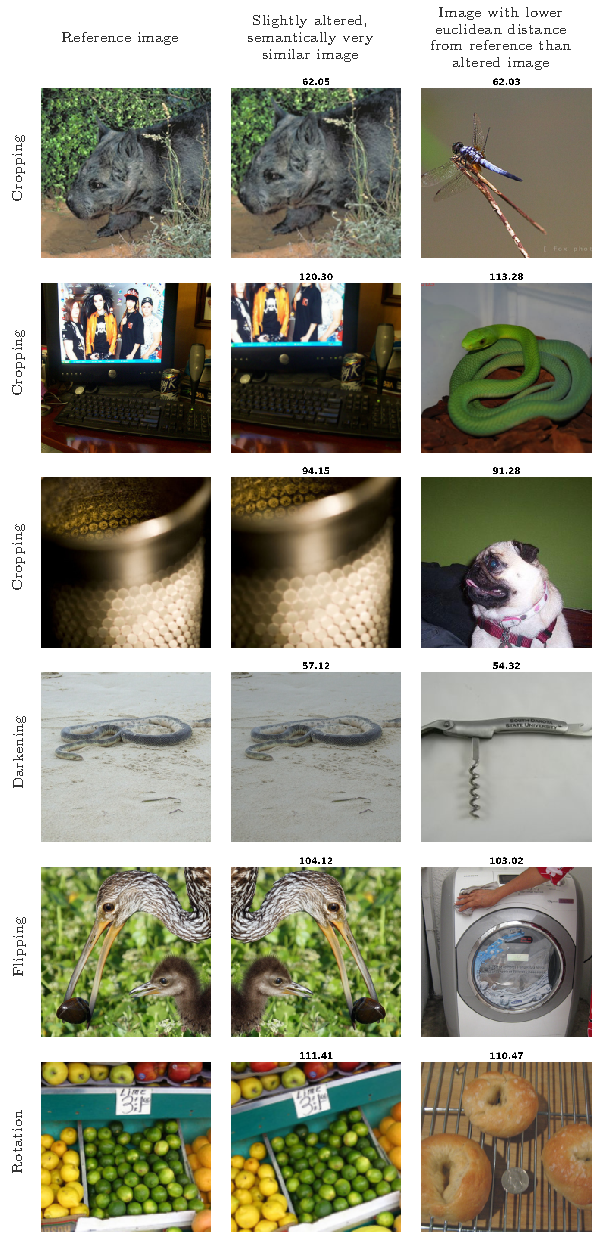
\includegraphics[width=.5\textwidth]{chapter4/figures/L2bad.pdf}
    \caption{Examples where the $L_2$-distance is not a (semantically) meaningful distance between images. In the left column, a reference image from ImageNet \citep{imagenet} is shown. In the middle column, a slight alteration is applied, whose result a human observer would consider to be very close to the reference image. In the right column, another image from the ImageNet data set is displayed, which to the human observer is very different from the reference image, but which has a lower $L_2$-distance to the reference image than the altered image. The numbers above the images indicate the $L_2$-distance to the reference image. Figure taken from \cite{stanczuk2021wasserstein}.}
    \label{ch4:fig:L2bad}
\end{figure}

\section{Experimental details} \label{ch4:Experimental_details}

\subsection{ScoreVAE}
The pretrained diffusion models for all experiments are based on the DDPM architecture \cite{ddpm}. We used $128$ base filters and attention at resolution $16\times 16$ for all experiments. For Cifar10, we set the channel multiplier array to $[1, 2, 2, 2]$ and the number of ResNet blocks to $4$. For CelebA $64\times 64$, we set the channel multiplier array to $[1, 1, 2, 2, 3]$ and the number of ResNet blocks to $2$. We used $0.1$ dropout rate for Cifar10 and $0$ dropout rate for CelebA. We used the beta-linear variance preserving forward process with the same parameters as the ones used by \cite{song2020score} and trained the diffusion model using the weighted denoising score matching objective with the simple weighting, i.e., $\lambda(t)=\sigma(t)^2$, where $\sigma(t)$ is the standard deviation of the perturbation kernel. We used the Adam optimizer and EMA rate 0.999. Finally, we set the learning rate to $2\mathrm{e}{-4}$ for Cifar10 and $1\mathrm{e}{-4}$ for CelebA.

The time dependent encoder for the Cifar10 experiment is a simple convolutional network that consists of a sequence of blocks of convolutions followed by the GELU activation function. The final activation is flattened and concatenated to the time tensor. A final linear layer maps the time augmented flattened tensor to the latent dimension. The time dependent encoder for CelebA is based heavily on the DDPM architecture. We removed the upsampling part of the U-NET and removed the skip connections. The downscaled tensor is flattened and mapped to the latent dimension with an additional linear layer. We used the Adam optimizer and EMA rate 0.999. We set the learning rate to $2\mathrm{e}{-4}$ for Cifar10 and $1\mathrm{e}{-4}$ for CelebA. We trained the Cifar10 encoder for $1.4M$ iterations and the CelebA encoder for $300K$ iterations.

\subsection{VAE}

For VAE we used exactly the same encoder architectures as in the Score VAE (except they were not conditioned on time). For each choice of encoder we created a mirror decoder with symmetric architecture. In Cifar10 the decoder starts by reshaping the the flat latent vector into a tensor which is then passed through a sequence of transposed convolutions which exactly mirror the structure of the encoder. In CelebA we used a decoder consisting of the upsampling part of the DDPM U-NET. The Cifar10 model was trained for 11M iterations, while the CelebA model was trained for 600K iterations.



\newpage
\section{Extended qualitative evaluation}\label{ch4:sec:extended_qualitative_evaluation}


\begin{table}[h!]
    \centering
    \resizebox{0.75\textwidth}{!}{
    \begin{tabular}{cccccc}
        Original & \multicolumn{1}{c}{ScoreVAE} & \multicolumn{1}{c}{ScoreVAE+} & \multicolumn{2}{c}{DiffDecoder} & \multicolumn{1}{c}{VAE}  \\ 
        & ($\beta=0.01$) & ($\beta=0.01$) & ($\beta=0.01$) & ($\beta=0$) & ($\beta=0.01$) \\

        \includegraphics[width=.145\textwidth]{chapter4/figures/images/cifar10/original/1.png} &   
        \includegraphics[width=.145\textwidth]{chapter4/figures/images/cifar10/reconstruction/1.png} &
        \includegraphics[width=.145\textwidth]{chapter4/figures/images/cifar10/corrected_reconstruction/1.png} &
        \includegraphics[width=.145\textwidth]{chapter4/figures/images/cifar10/diffusion_decoder_beta_0.01/1.png} &
        \includegraphics[width=.145\textwidth]{chapter4/figures/images/cifar10/diffusion_decoder_beta_0/1.png} &
        \includegraphics[width=.145\textwidth]{chapter4/figures/images/cifar10/VAE_reconstruction/1.png} \\

        
\includegraphics[width=.145\textwidth]{chapter4/figures/images/cifar10/original/2.png} &   
        
\includegraphics[width=.145\textwidth]{chapter4/figures/images/cifar10/reconstruction/2.png} &
        
\includegraphics[width=.145\textwidth]{chapter4/figures/images/cifar10/corrected_reconstruction/2.png} &
        
\includegraphics[width=.145\textwidth]{chapter4/figures/images/cifar10/diffusion_decoder_beta_0.01/2.png} &
        
\includegraphics[width=.145\textwidth]{chapter4/figures/images/cifar10/diffusion_decoder_beta_0/2.png} &
        
\includegraphics[width=.145\textwidth]{chapter4/figures/images/cifar10/VAE_reconstruction/2.png} \\
 
        
\includegraphics[width=.145\textwidth]{chapter4/figures/images/cifar10/original/3.png} &   
        
\includegraphics[width=.145\textwidth]{chapter4/figures/images/cifar10/reconstruction/3.png} &
        
\includegraphics[width=.145\textwidth]{chapter4/figures/images/cifar10/corrected_reconstruction/3.png} &
        
\includegraphics[width=.145\textwidth]{chapter4/figures/images/cifar10/diffusion_decoder_beta_0.01/3.png} &
        
\includegraphics[width=.145\textwidth]{chapter4/figures/images/cifar10/diffusion_decoder_beta_0/3.png} &
        
\includegraphics[width=.145\textwidth]{chapter4/figures/images/cifar10/VAE_reconstruction/3.png} \\

        \includegraphics[width=.145\textwidth]{chapter4/figures/images/cifar10/original/4.png} &   
        \includegraphics[width=.145\textwidth]{chapter4/figures/images/cifar10/reconstruction/4.png} &
        \includegraphics[width=.145\textwidth]{chapter4/figures/images/cifar10/corrected_reconstruction/4.png} &
        \includegraphics[width=.145\textwidth]{chapter4/figures/images/cifar10/diffusion_decoder_beta_0.01/4.png} &
        \includegraphics[width=.145\textwidth]{chapter4/figures/images/cifar10/diffusion_decoder_beta_0/4.png} &
        \includegraphics[width=.145\textwidth]{chapter4/figures/images/cifar10/VAE_reconstruction/4.png} \\
        \includegraphics[width=.145\textwidth]{chapter4/figures/images/cifar10/original/5.png} &   
        \includegraphics[width=.145\textwidth]{chapter4/figures/images/cifar10/reconstruction/5.png} &
        \includegraphics[width=.145\textwidth]{chapter4/figures/images/cifar10/corrected_reconstruction/5.png} &
        \includegraphics[width=.145\textwidth]{chapter4/figures/images/cifar10/diffusion_decoder_beta_0.01/5.png} &
        \includegraphics[width=.145\textwidth]{chapter4/figures/images/cifar10/diffusion_decoder_beta_0/5.png} &
        \includegraphics[width=.145\textwidth]{chapter4/figures/images/cifar10/VAE_reconstruction/5.png} \\
        \includegraphics[width=.145\textwidth]{chapter4/figures/images/cifar10/original/6.png} &   
        \includegraphics[width=.145\textwidth]{chapter4/figures/images/cifar10/reconstruction/6.png} &
        \includegraphics[width=.145\textwidth]{chapter4/figures/images/cifar10/corrected_reconstruction/6.png} &
        \includegraphics[width=.145\textwidth]{chapter4/figures/images/cifar10/diffusion_decoder_beta_0.01/6.png} &
        \includegraphics[width=.145\textwidth]{chapter4/figures/images/cifar10/diffusion_decoder_beta_0/6.png} &
        \includegraphics[width=.145\textwidth]{chapter4/figures/images/cifar10/VAE_reconstruction/6.png} \\
        
\includegraphics[width=.145\textwidth]{chapter4/figures/images/cifar10/original/7.png} &   
        
\includegraphics[width=.145\textwidth]{chapter4/figures/images/cifar10/reconstruction/7.png} &
        
\includegraphics[width=.145\textwidth]{chapter4/figures/images/cifar10/corrected_reconstruction/7.png} &
        
\includegraphics[width=.145\textwidth]{chapter4/figures/images/cifar10/diffusion_decoder_beta_0.01/7.png} &
        
\includegraphics[width=.145\textwidth]{chapter4/figures/images/cifar10/diffusion_decoder_beta_0/7.png} &
        
\includegraphics[width=.145\textwidth]{chapter4/figures/images/cifar10/VAE_reconstruction/7.png} \\
        \includegraphics[width=.145\textwidth]{chapter4/figures/images/cifar10/original/8.png} &   
        \includegraphics[width=.145\textwidth]{chapter4/figures/images/cifar10/reconstruction/8.png} &
        \includegraphics[width=.145\textwidth]{chapter4/figures/images/cifar10/corrected_reconstruction/8.png} &
        \includegraphics[width=.145\textwidth]{chapter4/figures/images/cifar10/diffusion_decoder_beta_0.01/8.png} &
        \includegraphics[width=.145\textwidth]{chapter4/figures/images/cifar10/diffusion_decoder_beta_0/8.png} &
        \includegraphics[width=.145\textwidth]{chapter4/figures/images/cifar10/VAE_reconstruction/8.png} \\
        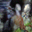
\includegraphics[width=.145\textwidth]{chapter4/figures/images/cifar10/original/9.png} &   
        \includegraphics[width=.145\textwidth]{chapter4/figures/images/cifar10/reconstruction/9.png} &
        \includegraphics[width=.145\textwidth]{chapter4/figures/images/cifar10/corrected_reconstruction/9.png} &
        \includegraphics[width=.145\textwidth]{chapter4/figures/images/cifar10/diffusion_decoder_beta_0.01/9.png} &
        \includegraphics[width=.145\textwidth]{chapter4/figures/images/cifar10/diffusion_decoder_beta_0/9.png} &
        \includegraphics[width=.145\textwidth]{chapter4/figures/images/cifar10/VAE_reconstruction/9.png} \\
        \includegraphics[width=.145\textwidth]{chapter4/figures/images/cifar10/original/10.png} &   
        \includegraphics[width=.145\textwidth]{chapter4/figures/images/cifar10/reconstruction/10.png} &
        \includegraphics[width=.145\textwidth]{chapter4/figures/images/cifar10/corrected_reconstruction/10.png} &
        \includegraphics[width=.145\textwidth]{chapter4/figures/images/cifar10/diffusion_decoder_beta_0.01/10.png} &
        \includegraphics[width=.145\textwidth]{chapter4/figures/images/cifar10/diffusion_decoder_beta_0/10.png} &
        \includegraphics[width=.145\textwidth]{chapter4/figures/images/cifar10/VAE_reconstruction/10.png} \\
        \includegraphics[width=.145\textwidth]{chapter4/figures/images/cifar10/original/11.png} &   
        \includegraphics[width=.145\textwidth]{chapter4/figures/images/cifar10/reconstruction/11.png} &
        \includegraphics[width=.145\textwidth]{chapter4/figures/images/cifar10/corrected_reconstruction/11.png} &
        \includegraphics[width=.145\textwidth]{chapter4/figures/images/cifar10/diffusion_decoder_beta_0.01/11.png} &
        \includegraphics[width=.145\textwidth]{chapter4/figures/images/cifar10/diffusion_decoder_beta_0/11.png} &
        \includegraphics[width=.145\textwidth]{chapter4/figures/images/cifar10/VAE_reconstruction/11.png} \\
    \end{tabular}}
    \caption{Cifar10}
    \label{ch4:fig:extended_cifar10_qualitative_comparison}
\end{table}


\begin{table}[h!]
    \centering
    \resizebox{0.9\textwidth}{!}{
    \begin{tabular}{cccccc}
        Original & \multicolumn{1}{c}{ScoreVAE} & \multicolumn{1}{c}{ScoreVAE+} & \multicolumn{2}{c}{DiffDecoder} & \multicolumn{1}{c}{VAE}  \\ 
        & ($\beta=0.01$) & ($\beta=0.01$) & ($\beta=0.01$) & ($\beta=0$) & ($\beta=0.01$) \\

        \includegraphics[width=.145\textwidth]{chapter4/figures/images/celebA/original/1.png} &   
        \includegraphics[width=.145\textwidth]{chapter4/figures/images/celebA/reconstruction/1.png} &
        \includegraphics[width=.145\textwidth]{chapter4/figures/images/celebA/corrected_reconstruction/1.png} &
        \includegraphics[width=.145\textwidth]{chapter4/figures/images/celebA/diffusion_decoder_beta_0.01/1.png} &
        \includegraphics[width=.145\textwidth]{chapter4/figures/images/celebA/diffusion_decoder_beta_0/1.png} &
        \includegraphics[width=.145\textwidth]{chapter4/figures/images/celebA/VAE_reconstruction/1.png} \\

        \includegraphics[width=.145\textwidth]{chapter4/figures/images/celebA/original/2.png} &   
        \includegraphics[width=.145\textwidth]{chapter4/figures/images/celebA/reconstruction/2.png} &
        \includegraphics[width=.145\textwidth]{chapter4/figures/images/celebA/corrected_reconstruction/2.png} &
        \includegraphics[width=.145\textwidth]{chapter4/figures/images/celebA/diffusion_decoder_beta_0.01/2.png} &
        \includegraphics[width=.145\textwidth]{chapter4/figures/images/celebA/diffusion_decoder_beta_0/2.png} &
        \includegraphics[width=.145\textwidth]{chapter4/figures/images/celebA/VAE_reconstruction/2.png} \\
 
        \includegraphics[width=.145\textwidth]{chapter4/figures/images/celebA/original/3.png} &   
        \includegraphics[width=.145\textwidth]{chapter4/figures/images/celebA/reconstruction/3.png} &
        \includegraphics[width=.145\textwidth]{chapter4/figures/images/celebA/corrected_reconstruction/3.png} &
        \includegraphics[width=.145\textwidth]{chapter4/figures/images/celebA/diffusion_decoder_beta_0.01/3.png} &
        \includegraphics[width=.145\textwidth]{chapter4/figures/images/celebA/diffusion_decoder_beta_0/3.png} &
        \includegraphics[width=.145\textwidth]{chapter4/figures/images/celebA/VAE_reconstruction/3.png} \\

        \includegraphics[width=.145\textwidth]{chapter4/figures/images/celebA/original/4.png} &   
        \includegraphics[width=.145\textwidth]{chapter4/figures/images/celebA/reconstruction/4.png} &
        \includegraphics[width=.145\textwidth]{chapter4/figures/images/celebA/corrected_reconstruction/4.png} &
        \includegraphics[width=.145\textwidth]{chapter4/figures/images/celebA/diffusion_decoder_beta_0.01/4.png} &
        \includegraphics[width=.145\textwidth]{chapter4/figures/images/celebA/diffusion_decoder_beta_0/4.png} &
        \includegraphics[width=.145\textwidth]{chapter4/figures/images/celebA/VAE_reconstruction/4.png} \\
        \includegraphics[width=.145\textwidth]{chapter4/figures/images/celebA/original/5.png} &   
        \includegraphics[width=.145\textwidth]{chapter4/figures/images/celebA/reconstruction/5.png} &
        \includegraphics[width=.145\textwidth]{chapter4/figures/images/celebA/corrected_reconstruction/5.png} &
        \includegraphics[width=.145\textwidth]{chapter4/figures/images/celebA/diffusion_decoder_beta_0.01/5.png} &
        \includegraphics[width=.145\textwidth]{chapter4/figures/images/celebA/diffusion_decoder_beta_0/5.png} &
        \includegraphics[width=.145\textwidth]{chapter4/figures/images/celebA/VAE_reconstruction/5.png} \\
        \includegraphics[width=.145\textwidth]{chapter4/figures/images/celebA/original/6.png} &   
        \includegraphics[width=.145\textwidth]{chapter4/figures/images/celebA/reconstruction/6.png} &
        \includegraphics[width=.145\textwidth]{chapter4/figures/images/celebA/corrected_reconstruction/6.png} &
        \includegraphics[width=.145\textwidth]{chapter4/figures/images/celebA/diffusion_decoder_beta_0.01/6.png} &
        \includegraphics[width=.145\textwidth]{chapter4/figures/images/celebA/diffusion_decoder_beta_0/6.png} &
        \includegraphics[width=.145\textwidth]{chapter4/figures/images/celebA/VAE_reconstruction/6.png} \\
        \includegraphics[width=.145\textwidth]{chapter4/figures/images/celebA/original/7.png} &   
        \includegraphics[width=.145\textwidth]{chapter4/figures/images/celebA/reconstruction/7.png} &
        \includegraphics[width=.145\textwidth]{chapter4/figures/images/celebA/corrected_reconstruction/7.png} &
        \includegraphics[width=.145\textwidth]{chapter4/figures/images/celebA/diffusion_decoder_beta_0.01/7.png} &
        \includegraphics[width=.145\textwidth]{chapter4/figures/images/celebA/diffusion_decoder_beta_0/7.png} &
        \includegraphics[width=.145\textwidth]{chapter4/figures/images/celebA/VAE_reconstruction/7.png} \\
        \includegraphics[width=.145\textwidth]{chapter4/figures/images/celebA/original/8.png} &   
        \includegraphics[width=.145\textwidth]{chapter4/figures/images/celebA/reconstruction/8.png} &
        \includegraphics[width=.145\textwidth]{chapter4/figures/images/celebA/corrected_reconstruction/8.png} &
        \includegraphics[width=.145\textwidth]{chapter4/figures/images/celebA/diffusion_decoder_beta_0.01/8.png} &
        \includegraphics[width=.145\textwidth]{chapter4/figures/images/celebA/diffusion_decoder_beta_0/8.png} &
        \includegraphics[width=.145\textwidth]{chapter4/figures/images/celebA/VAE_reconstruction/8.png} \\
        \includegraphics[width=.145\textwidth]{chapter4/figures/images/celebA/original/9.png} &   
        \includegraphics[width=.145\textwidth]{chapter4/figures/images/celebA/reconstruction/9.png} &
        \includegraphics[width=.145\textwidth]{chapter4/figures/images/celebA/corrected_reconstruction/9.png} &
        \includegraphics[width=.145\textwidth]{chapter4/figures/images/celebA/diffusion_decoder_beta_0.01/9.png} &
        \includegraphics[width=.145\textwidth]{chapter4/figures/images/celebA/diffusion_decoder_beta_0/9.png} &
        \includegraphics[width=.145\textwidth]{chapter4/figures/images/celebA/VAE_reconstruction/9.png} \\
        \includegraphics[width=.145\textwidth]{chapter4/figures/images/celebA/original/10.png} &   
        \includegraphics[width=.145\textwidth]{chapter4/figures/images/celebA/reconstruction/10.png} &
        \includegraphics[width=.145\textwidth]{chapter4/figures/images/celebA/corrected_reconstruction/10.png} &
        \includegraphics[width=.145\textwidth]{chapter4/figures/images/celebA/diffusion_decoder_beta_0.01/10.png} &
        \includegraphics[width=.145\textwidth]{chapter4/figures/images/celebA/diffusion_decoder_beta_0/10.png} &
        \includegraphics[width=.145\textwidth]{chapter4/figures/images/celebA/VAE_reconstruction/10.png} \\
        \includegraphics[width=.145\textwidth]{chapter4/figures/images/celebA/original/11.png} &   
        \includegraphics[width=.145\textwidth]{chapter4/figures/images/celebA/reconstruction/11.png} &
        \includegraphics[width=.145\textwidth]{chapter4/figures/images/celebA/corrected_reconstruction/11.png} &
        \includegraphics[width=.145\textwidth]{chapter4/figures/images/celebA/diffusion_decoder_beta_0.01/11.png} &
        \includegraphics[width=.145\textwidth]{chapter4/figures/images/celebA/diffusion_decoder_beta_0/11.png} &
        \includegraphics[width=.145\textwidth]{chapter4/figures/images/celebA/VAE_reconstruction/11.png} \\
    \end{tabular}}
    \caption{CelebA}
    \label{ch4:fig:extended_celebA_qualitative_comparison}
\end{table}